\documentclass{article}

%{
%  \usetheme{default}      
%  \usecolortheme{default}
%  \usefonttheme{default}  
%  \setbeamertemplate{navigation symbols}{}
%  \setbeamertemplate{caption}[numbered]
%  \setbeamertemplate{footline}[frame number]
%} 

\usepackage[english]{babel}
\usepackage[utf8x]{inputenc}
\usepackage{amsthm, amssymb, amsfonts, amsmath}
\usepackage{graphicx}
\usepackage{float}
\usepackage{lscape}
\usepackage{tikz}
\usetikzlibrary{calc,shapes}
\usepackage{mathtools}
\usepackage{mathrsfs}
\usepackage{tikz-cd}
\usetikzlibrary{positioning}
\usepackage{courier}
\usepackage{xcolor}
\usepackage{booktabs}
\usepackage{caption}
\usepackage[doublespacing]{setspace}
\usepackage{url}
\usepackage{subcaption}
%\pagestyle{empty} 		% This supresses the page numbers
\usepackage[authoryear]{natbib}
\usepackage{natbib} %Fundamental for good referencing, you also have to remember harvard.bst, for Harvard style refs.
\usepackage{hyperref}
\hypersetup{colorlinks=true, urlcolor=blue, linkcolor=blue, citecolor=blue}

\newcommand{\comment}[1]{{\color{red}#1}}

\newcommand{\rot}[2]{\rule{1em}{0pt}%
\makebox[0cm][c]{\rotatebox{#1}{\ #2}}}
\newcommand{\sym}[1]{\rlap{#1}}

\usepackage{siunitx} % centering in tables
	\sisetup{
		detect-mode,
		tight-spacing		= true,
		group-digits		= false ,
		input-signs		= ,
		input-symbols		= ( ) [ ] - + *,
		input-open-uncertainty	= ,
		input-close-uncertainty	= ,
		table-align-text-post	= false
        }

\newcolumntype{$}{>{\global\let\currentrowstyle\relax}}
\newcolumntype{^}{>{\currentrowstyle}}
\newcommand{\rowstyle}[1]{\gdef\currentrowstyle{#1}%
  #1\ignorespaces
}
%$


\title{Additional analysis - $G \times E$ paper}


\begin{document}
\maketitle


\bigskip 
Main differences from estimates in paper on overleaf:
\begin{itemize}
\item These include a YoB1992 dummy 
\item These include interactions a la Keller
\end{itemize}




\section{Predictive power of different PGSs}

\begin{table}[H]
\caption{Comparison of predictive power from PGSs}
\centering
{\footnotesize
\begin{tabular}{lcccccccccccccccccccc}
\toprule
            &\multicolumn{1}{c}{PLINK}&\multicolumn{1}{c}{UKB}&\multicolumn{2}{c}{23\&me}                 \\\cmidrule(lr){2-2}\cmidrule(lr){3-3}\cmidrule(lr){4-5}
            &\multicolumn{1}{c}{(1)}         &\multicolumn{1}{c}{(2)}         &\multicolumn{1}{c}{(3)}         &\multicolumn{1}{c}{(4)}         \\
\midrule
PGS         &       0.290\sym{***}&       0.319\sym{***}&       0.285\sym{***}&       0.344\sym{***}\\
            &     (0.015)         &     (0.015)         &     (0.015)         &     (0.015)         \\
\midrule
R2          &       0.089         &       0.109         &       0.086         &       0.124         \\
Observations&        3610         &        3610         &        3610         &        3610         \\

\bottomrule
\addlinespace[.75ex]
\end{tabular}
}
\caption*{\noindent\scriptsize Robust standard errors in parentheses. * $p < 0.1$, ** $p < 0.05$, *** $p < 0.01$.}
\end{table}

\clearpage


\section{MoB analysis with different PGSs}
\begin{table}[H]
\caption{Entry Assessment (age 4) test; using Plink-based PGS}
\centering
{\scriptsize
\begin{tabular}{lcccccccccccccccccccc}
\toprule
            &\multicolumn{1}{c}{(1)}         &\multicolumn{1}{c}{(2)}         \\
\midrule
Treated     &       1.054\sym{***}&       0.859\sym{***}\\
            &     (0.074)         &     (0.065)         \\
\addlinespace
Treated*PGS &                     &      -0.280\sym{***}\\
            &                     &     (0.048)         \\
\addlinespace
Treated*MoB &       0.058         &       0.083         \\
            &     (0.049)         &     (0.056)         \\
\addlinespace
MoB*PGS     &                     &      -0.084\sym{***}\\
            &                     &     (0.010)         \\
\addlinespace
MoB*PGS*Treated&                     &       0.162\sym{***}\\
            &                     &     (0.019)         \\
\addlinespace
MoB         &      -0.144\sym{**} &      -0.156\sym{**} \\
            &     (0.050)         &     (0.049)         \\
\addlinespace
PGS         &       0.164\sym{***}&       0.193\sym{***}\\
            &     (0.037)         &     (0.029)         \\
\midrule
R2          &       0.248         &       0.264         \\
Observations&        1094         &        1094         \\

\bottomrule
\addlinespace[.75ex]
\end{tabular}
}
\caption*{\noindent\scriptsize Robust standard errors clustered by month of birth in parentheses. * $p < 0.1$, ** $p < 0.05$, *** $p < 0.01$.}
\end{table}

\begin{table}[H]
\caption{Key Stage tests; using Plink-based PGS}
\centering
{\scriptsize
\begin{tabular}{lcccccccccccccccccccc}
\toprule
            &\multicolumn{2}{c}{Key Stage 1}            &\multicolumn{2}{c}{Key Stage 2}            &\multicolumn{2}{c}{Key Stage 3}            &\multicolumn{2}{c}{Key Stage 4}            \\\cmidrule(lr){2-3}\cmidrule(lr){4-5}\cmidrule(lr){6-7}\cmidrule(lr){8-9}
\midrule
Treated     &       0.590\sym{***}&       0.626\sym{***}&       0.211\sym{***}&       0.159\sym{***}&       0.142         &       0.159\sym{**} &       0.193\sym{***}&       0.223\sym{***}\\
            &     (0.016)         &     (0.052)         &     (0.017)         &     (0.037)         &     (0.081)         &     (0.058)         &     (0.032)         &     (0.034)         \\
\addlinespace
Treated*PGS &                     &      -0.084\sym{**} &                     &      -0.061\sym{*}  &                     &      -0.090\sym{***}&                     &      -0.015         \\
            &                     &     (0.030)         &                     &     (0.026)         &                     &     (0.019)         &                     &     (0.014)         \\
\addlinespace
Treated*MoB &       0.070\sym{***}&       0.068\sym{***}&       0.109\sym{***}&       0.110\sym{***}&       0.044         &       0.048         &       0.048\sym{**} &       0.046\sym{**} \\
            &     (0.011)         &     (0.011)         &     (0.013)         &     (0.012)         &     (0.030)         &     (0.031)         &     (0.015)         &     (0.016)         \\
\addlinespace
MoB*PGS     &                     &       0.013         &                     &       0.007         &                     &       0.033\sym{***}&                     &       0.045\sym{***}\\
            &                     &     (0.006)         &                     &     (0.009)         &                     &     (0.006)         &                     &     (0.009)         \\
\addlinespace
MoB*PGS*Treated&                     &       0.014         &                     &       0.014         &                     &       0.013         &                     &      -0.036\sym{**} \\
            &                     &     (0.009)         &                     &     (0.012)         &                     &     (0.008)         &                     &     (0.010)         \\
\addlinespace
MoB         &      -0.090\sym{***}&      -0.085\sym{***}&      -0.099\sym{***}&      -0.102\sym{***}&      -0.028         &      -0.026         &      -0.042\sym{**} &      -0.042\sym{**} \\
            &     (0.010)         &     (0.011)         &     (0.012)         &     (0.010)         &     (0.015)         &     (0.014)         &     (0.012)         &     (0.012)         \\
\addlinespace
PGS         &       0.237\sym{***}&       0.229\sym{***}&       0.293\sym{***}&       0.301\sym{***}&       0.316\sym{***}&       0.312\sym{***}&       0.276\sym{***}&       0.283\sym{***}\\
            &     (0.010)         &     (0.026)         &     (0.009)         &     (0.015)         &     (0.017)         &     (0.023)         &     (0.012)         &     (0.029)         \\
\midrule
R2          &       0.162         &       0.167         &       0.111         &       0.114         &       0.116         &       0.119         &       0.115         &       0.120         \\
Observations&        3436         &        3436         &        3610         &        3610         &        3073         &        3073         &        3579         &        3579         \\

\bottomrule
\addlinespace[.75ex]
\end{tabular}
}
\caption*{\noindent\scriptsize Robust standard errors clustered by month of birth in parentheses. * $p < 0.1$, ** $p < 0.05$, *** $p < 0.01$.}
\end{table}


\clearpage

\section{LDpred-based PGS using UKB sum stats}

\begin{table}[H]
\caption{Entry Assessment (age 4) test; using LDpred-based PGS with UKB sum stats}
\centering
{\scriptsize
\begin{tabular}{lcccccccccccccccccccc}
\toprule
            &\multicolumn{1}{c}{(1)}         &\multicolumn{1}{c}{(2)}         \\
\midrule
Treated     &       1.055\sym{***}&       0.889\sym{***}\\
            &     (0.080)         &     (0.084)         \\
\addlinespace
Treated*PGS &                     &      -0.090         \\
            &                     &     (0.078)         \\
\addlinespace
Treated*MoB &       0.057         &       0.066         \\
            &     (0.047)         &     (0.049)         \\
\addlinespace
MoB*PGS     &                     &      -0.066\sym{***}\\
            &                     &     (0.015)         \\
\addlinespace
MoB*PGS*Treated&                     &       0.106\sym{**} \\
            &                     &     (0.030)         \\
\addlinespace
MoB         &      -0.146\sym{**} &      -0.145\sym{**} \\
            &     (0.046)         &     (0.043)         \\
\addlinespace
PGS         &       0.161\sym{***}&       0.161\sym{**} \\
            &     (0.024)         &     (0.059)         \\
\midrule
R2          &       0.247         &       0.260         \\
Observations&        1094         &        1094         \\

\bottomrule
\addlinespace[.75ex]
\end{tabular}
}
\caption*{\noindent\scriptsize Robust standard errors clustered by month of birth in parentheses. * $p < 0.1$, ** $p < 0.05$, *** $p < 0.01$.}
\end{table}

\begin{table}[H]
\caption{Key Stage tests; using LDpred-based PGS with UKB sum stats}
\centering
{\scriptsize
\begin{tabular}{lcccccccccccccccccccc}
\toprule
            &\multicolumn{2}{c}{Key Stage 1}            &\multicolumn{2}{c}{Key Stage 2}            &\multicolumn{2}{c}{Key Stage 3}            &\multicolumn{2}{c}{Key Stage 4}            \\\cmidrule(lr){2-3}\cmidrule(lr){4-5}\cmidrule(lr){6-7}\cmidrule(lr){8-9}
\midrule
Treated     &       0.619\sym{***}&       0.658\sym{***}&       0.249\sym{***}&       0.189\sym{***}&       0.177\sym{*}  &       0.211\sym{**} &       0.232\sym{***}&       0.257\sym{***}\\
            &     (0.018)         &     (0.056)         &     (0.012)         &     (0.040)         &     (0.078)         &     (0.054)         &     (0.026)         &     (0.033)         \\
\addlinespace
Treated*PGS &                     &       0.007         &                     &      -0.023         &                     &      -0.034         &                     &       0.014         \\
            &                     &     (0.036)         &                     &     (0.047)         &                     &     (0.071)         &                     &     (0.013)         \\
\addlinespace
Treated*MoB &       0.067\sym{***}&       0.061\sym{***}&       0.101\sym{***}&       0.102\sym{***}&       0.033         &       0.034         &       0.038\sym{**} &       0.037\sym{**} \\
            &     (0.012)         &     (0.013)         &     (0.012)         &     (0.010)         &     (0.029)         &     (0.033)         &     (0.013)         &     (0.011)         \\
\addlinespace
MoB*PGS     &                     &       0.043\sym{***}&                     &       0.028         &                     &      -0.012         &                     &       0.025\sym{***}\\
            &                     &     (0.006)         &                     &     (0.015)         &                     &     (0.014)         &                     &     (0.003)         \\
\addlinespace
MoB*PGS*Treated&                     &      -0.037\sym{**} &                     &      -0.015         &                     &       0.038         &                     &      -0.027\sym{**} \\
            &                     &     (0.012)         &                     &     (0.019)         &                     &     (0.021)         &                     &     (0.007)         \\
\addlinespace
MoB         &      -0.097\sym{***}&      -0.091\sym{***}&      -0.107\sym{***}&      -0.107\sym{***}&      -0.031\sym{*}  &      -0.030\sym{*}  &      -0.046\sym{***}&      -0.046\sym{***}\\
            &     (0.012)         &     (0.013)         &     (0.010)         &     (0.009)         &     (0.013)         &     (0.014)         &     (0.011)         &     (0.011)         \\
\addlinespace
PGS         &       0.257\sym{***}&       0.232\sym{***}&       0.320\sym{***}&       0.308\sym{***}&       0.331\sym{***}&       0.315\sym{***}&       0.293\sym{***}&       0.291\sym{***}\\
            &     (0.015)         &     (0.021)         &     (0.013)         &     (0.038)         &     (0.016)         &     (0.053)         &     (0.007)         &     (0.023)         \\
\midrule
R2          &       0.173         &       0.183         &       0.129         &       0.136         &       0.126         &       0.130         &       0.126         &       0.129         \\
Observations&        3436         &        3436         &        3610         &        3610         &        3073         &        3073         &        3579         &        3579         \\

\bottomrule
\addlinespace[.75ex]
\end{tabular}
}
\caption*{\noindent\scriptsize Robust standard errors clustered by month of birth in parentheses. * $p < 0.1$, ** $p < 0.05$, *** $p < 0.01$.}
\end{table}


\clearpage

\section{LDpred-based PGS using 23\&me sum stats}

\begin{table}[H]
\caption{Entry Assessment (age 4) test; using LDpred-based PGS with 23\&me sum stats}
\centering
{\scriptsize
\begin{tabular}{lcccccccccccccccccccc}
\toprule
            &\multicolumn{1}{c}{(1)}         &\multicolumn{1}{c}{(2)}         \\
\midrule
Treated     &       1.052\sym{***}&       0.882\sym{***}\\
            &     (0.064)         &     (0.057)         \\
\addlinespace
Treated*PGS &                     &      -0.145\sym{**} \\
            &                     &     (0.051)         \\
\addlinespace
Treated*MoB &       0.054         &       0.077         \\
            &     (0.045)         &     (0.047)         \\
\addlinespace
MoB*PGS     &                     &      -0.047\sym{**} \\
            &                     &     (0.015)         \\
\addlinespace
MoB*PGS*Treated&                     &       0.106\sym{***}\\
            &                     &     (0.025)         \\
\addlinespace
MoB         &      -0.141\sym{**} &      -0.158\sym{**} \\
            &     (0.046)         &     (0.043)         \\
\addlinespace
PGS         &       0.119\sym{***}&       0.126\sym{***}\\
            &     (0.025)         &     (0.024)         \\
\midrule
R2          &       0.237         &       0.251         \\
Observations&        1094         &        1094         \\

\bottomrule
\addlinespace[.75ex]
\end{tabular}
}
\caption*{\noindent\scriptsize Robust standard errors clustered by month of birth in parentheses. * $p < 0.1$, ** $p < 0.05$, *** $p < 0.01$.}
\end{table}

\begin{table}[H]
\caption{Key Stage tests; using LDpred-based PGS with 23\&me sum stats}
\centering
{\scriptsize
\begin{tabular}{lcccccccccccccccccccc}
\toprule
            &\multicolumn{2}{c}{Key Stage 1}            &\multicolumn{2}{c}{Key Stage 2}            &\multicolumn{2}{c}{Key Stage 3}            &\multicolumn{2}{c}{Key Stage 4}            \\\cmidrule(lr){2-3}\cmidrule(lr){4-5}\cmidrule(lr){6-7}\cmidrule(lr){8-9}
\midrule
Treated     &       0.620\sym{***}&       0.658\sym{***}&       0.262\sym{***}&       0.202\sym{***}&       0.188         &       0.243\sym{**} &       0.241\sym{***}&       0.263\sym{***}\\
            &     (0.019)         &     (0.046)         &     (0.031)         &     (0.031)         &     (0.098)         &     (0.083)         &     (0.043)         &     (0.041)         \\
\addlinespace
Treated*PGS &                     &      -0.112\sym{**} &                     &      -0.069\sym{***}&                     &      -0.049\sym{**} &                     &      -0.041         \\
            &                     &     (0.038)         &                     &     (0.008)         &                     &     (0.016)         &                     &     (0.025)         \\
\addlinespace
Treated*MoB &       0.056\sym{***}&       0.052\sym{**} &       0.082\sym{***}&       0.081\sym{***}&       0.015         &       0.009         &       0.023         &       0.021         \\
            &     (0.012)         &     (0.014)         &     (0.016)         &     (0.015)         &     (0.036)         &     (0.036)         &     (0.018)         &     (0.018)         \\
\addlinespace
MoB*PGS     &                     &       0.048\sym{***}&                     &       0.012         &                     &       0.009         &                     &       0.022\sym{***}\\
            &                     &     (0.012)         &                     &     (0.010)         &                     &     (0.007)         &                     &     (0.003)         \\
\addlinespace
MoB*PGS*Treated&                     &      -0.006         &                     &       0.012         &                     &       0.037\sym{***}&                     &      -0.003         \\
            &                     &     (0.015)         &                     &     (0.009)         &                     &     (0.005)         &                     &     (0.011)         \\
\addlinespace
MoB         &      -0.087\sym{***}&      -0.083\sym{***}&      -0.091\sym{***}&      -0.092\sym{***}&      -0.016         &      -0.014         &      -0.033\sym{**} &      -0.033\sym{**} \\
            &     (0.012)         &     (0.013)         &     (0.012)         &     (0.009)         &     (0.015)         &     (0.013)         &     (0.012)         &     (0.011)         \\
\addlinespace
PGS         &       0.210\sym{***}&       0.197\sym{***}&       0.287\sym{***}&       0.275\sym{***}&       0.304\sym{***}&       0.253\sym{***}&       0.274\sym{***}&       0.249\sym{***}\\
            &     (0.020)         &     (0.013)         &     (0.010)         &     (0.024)         &     (0.021)         &     (0.023)         &     (0.007)         &     (0.019)         \\
\midrule
R2          &       0.149         &       0.153         &       0.106         &       0.108         &       0.106         &       0.110         &       0.113         &       0.116         \\
Observations&        3436         &        3436         &        3610         &        3610         &        3073         &        3073         &        3579         &        3579         \\

\bottomrule
\addlinespace[.75ex]
\end{tabular}
}
\caption*{\noindent\scriptsize Robust standard errors clustered by month of birth in parentheses. * $p < 0.1$, ** $p < 0.05$, *** $p < 0.01$.}
\end{table}

\clearpage


\section{Parental investments }

\begin{figure}[H]
  \centering
  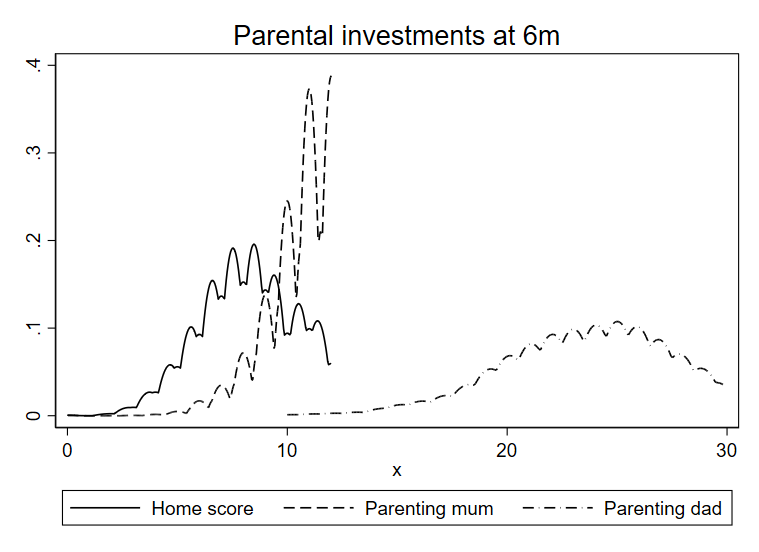
\includegraphics[width=0.45\linewidth]{../figures/Investments1_unadj.png}
  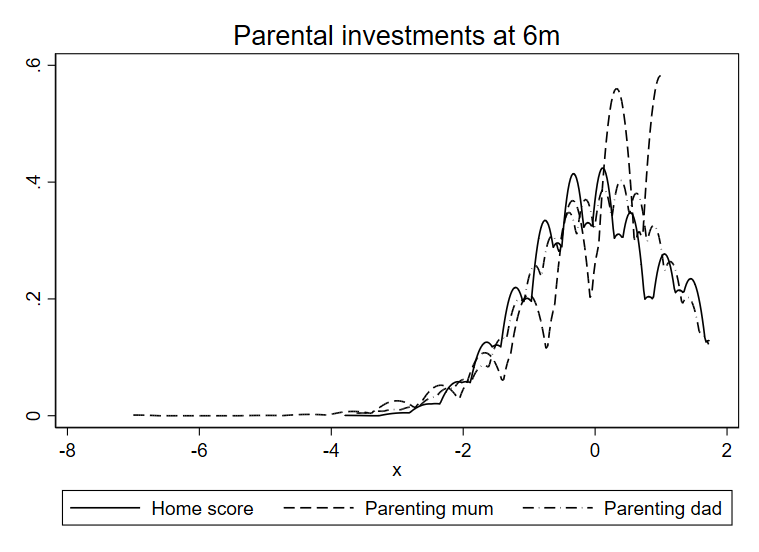
\includegraphics[width=0.45\linewidth]{../figures/Investments1.png} \\
  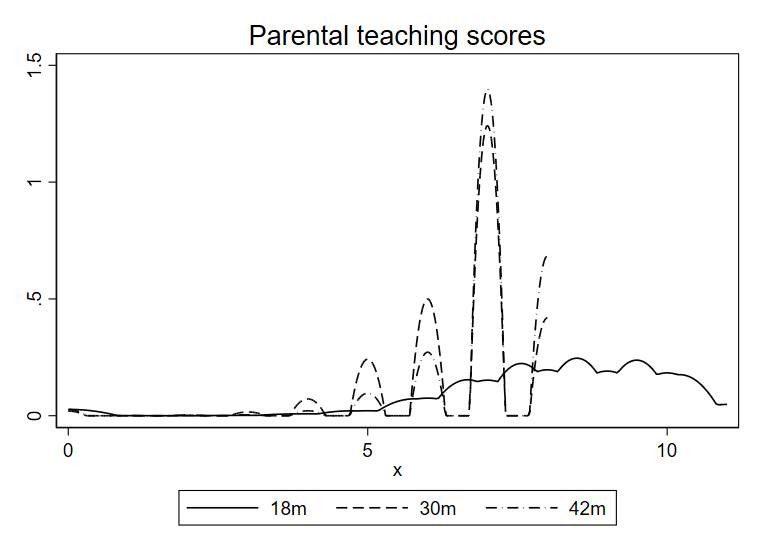
\includegraphics[width=0.45\linewidth]{../figures/Investments2_unadj.png} 
  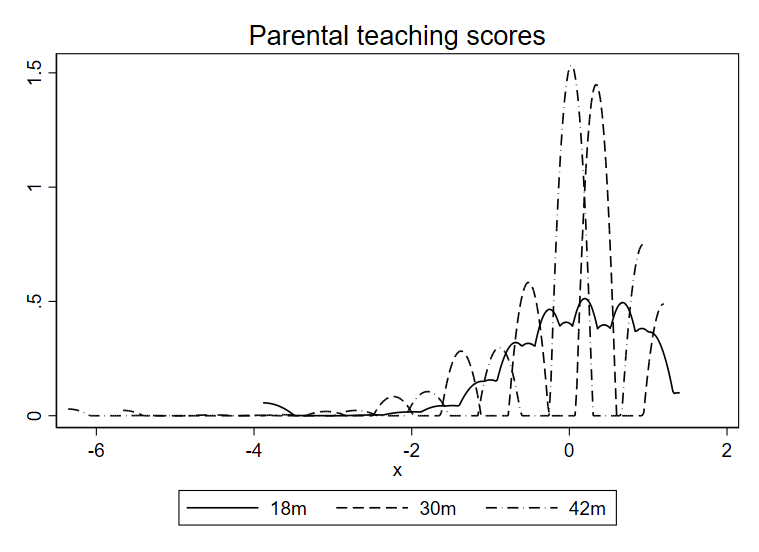
\includegraphics[width=0.45\linewidth]{../figures/Investments2.png} 
  \caption{Distribution of the parental investments scores (original and standardized}
\end{figure}

\begin{figure}[H]
\centering 
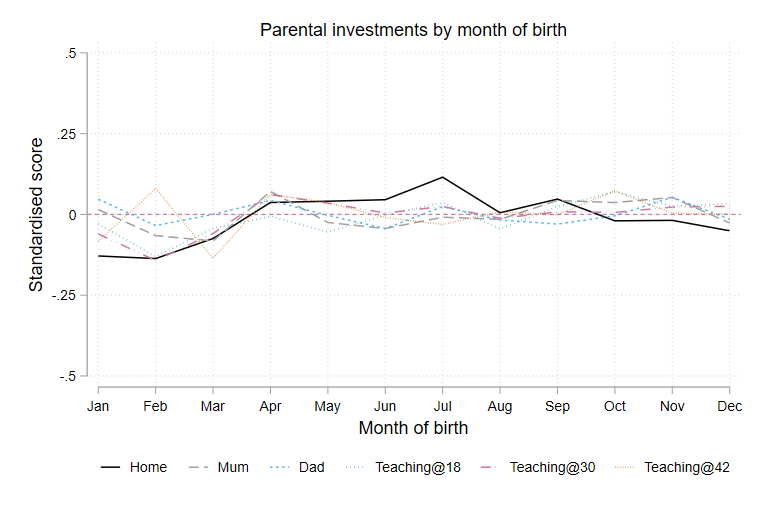
\includegraphics[width=1\linewidth]{../figures/Invest_MoB.png}
\caption{Parental investments by month of birth.}
\label{fig:Invest_MoB}
\end{figure}

\begin{figure}[H]
\centering 
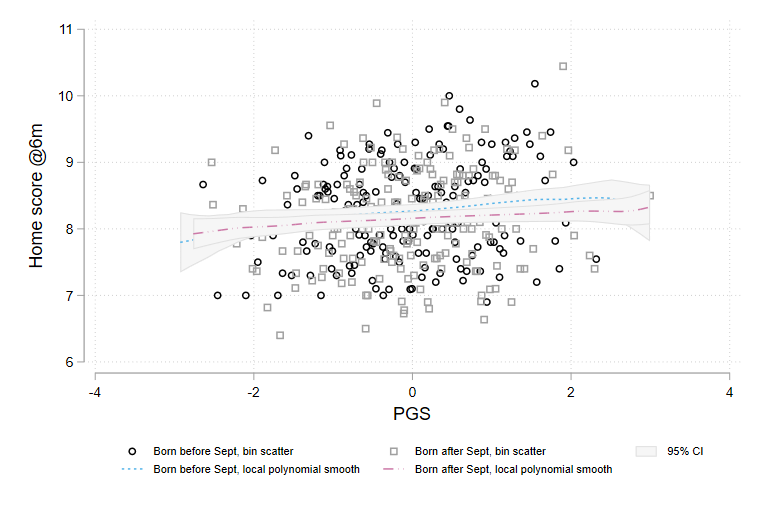
\includegraphics[width=1\linewidth]{../figures/PGSxTreat_home.png}
\caption{Relationship between PGS and investment (home score) by treated/control.}
\label{fig:PGSxTreat_home}
\end{figure}

\begin{figure}[H]
\centering 
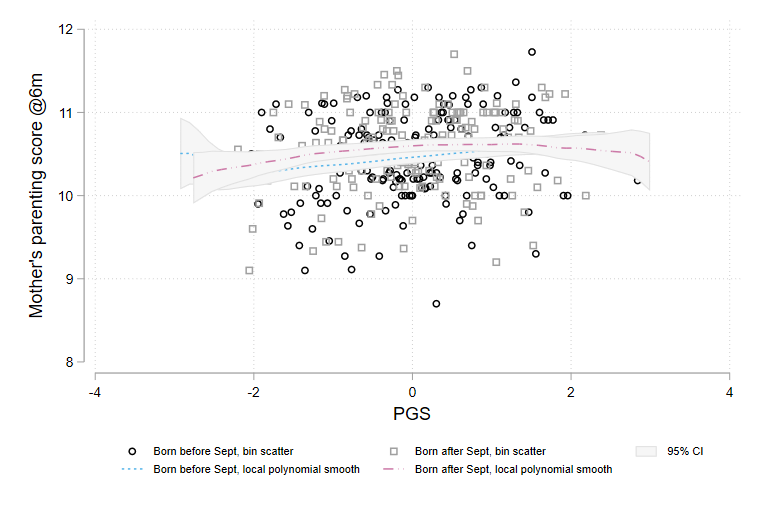
\includegraphics[width=1\linewidth]{../figures/PGSxTreat_mumpar.png}
\caption{Relationship between PGS and investment (mum parenting score) by treated/control.}
\label{fig:PGSxTreat_mumpar}
\end{figure}

\begin{figure}[H]
\centering 
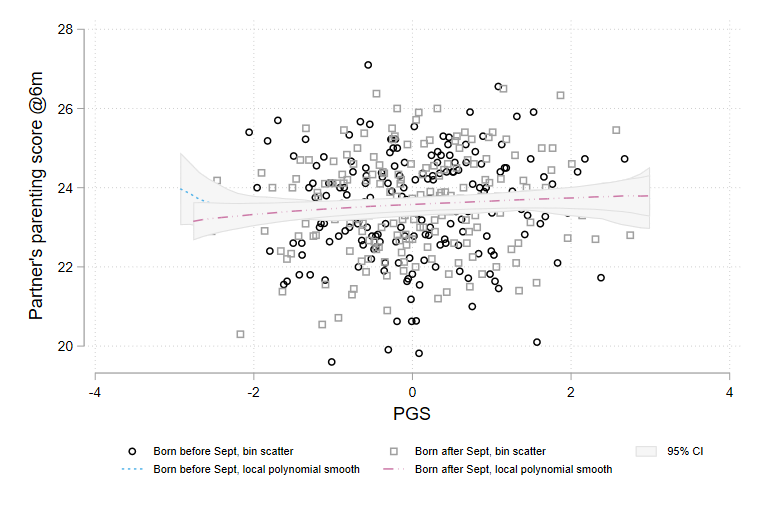
\includegraphics[width=1\linewidth]{../figures/PGSxTreat_dadpar.png}
\caption{Relationship between PGS and investment (dad parenting score) by treated/control.}
\label{fig:PGSxTreat_dadpar}
\end{figure}

\begin{figure}[H]
\centering 
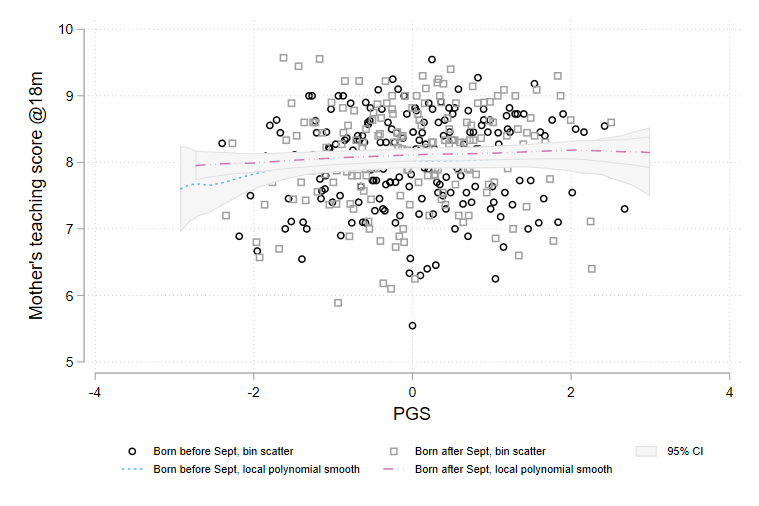
\includegraphics[width=1\linewidth]{../figures/PGSxTreat_teach18m.png}
\caption{Relationship between PGS and investment (teaching score 18m) by treated/control.}
\label{fig:PGSxTreat_teach18m}
\end{figure}

\begin{figure}[H]
\centering 
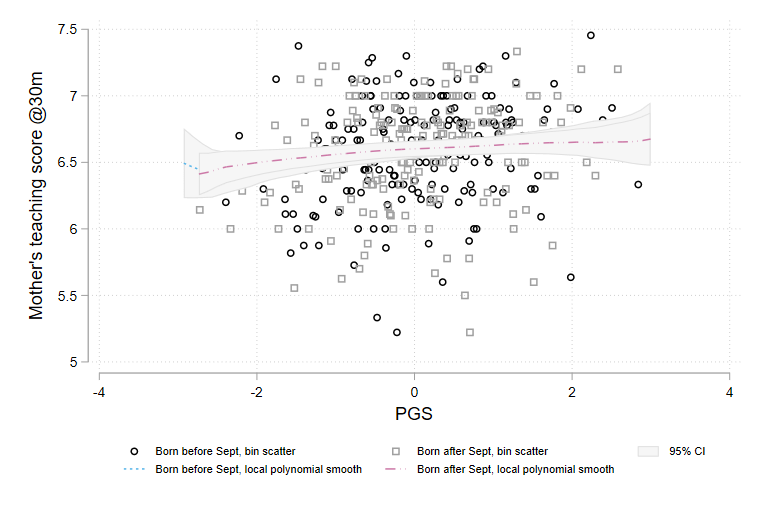
\includegraphics[width=1\linewidth]{../figures/PGSxTreat_teach30m.png}
\caption{Relationship between PGS and investment (teaching score 30m) by treated/control.}
\label{fig:PGSxTreat_teach30m}
\end{figure}

\begin{figure}[H]
\centering 
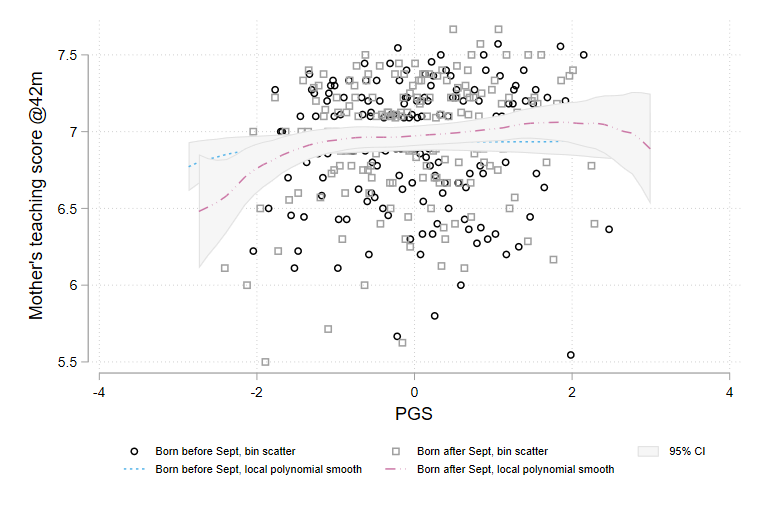
\includegraphics[width=1\linewidth]{../figures/PGSxTreat_teach42m.png}
\caption{Relationship between PGS and investment (teaching score 42m) by treated/control.}
\label{fig:PGSxTreat_teach42m}
\end{figure}



\section{Parental investments at 6 months}
All tables here on EA sample - results generally similar on larger (KS2) sample, esp for teaching scores (estimates for 6m home/parenting scores are more variable)

\begin{table}[H]
\caption{Investments at 6m; using Plink-based PGS (EA sample)}
\centering
{\scriptsize
\begin{tabular}{lcccccccccccccccccccc}
\toprule
            &\multicolumn{1}{c}{Home score @6m}&\multicolumn{1}{c}{Parenting Mum @6m}&\multicolumn{1}{c}{Parenting Dad @6m}\\\cmidrule(lr){2-2}\cmidrule(lr){3-3}\cmidrule(lr){4-4}
            &\multicolumn{1}{c}{(1)}         &\multicolumn{1}{c}{(2)}         &\multicolumn{1}{c}{(3)}         \\
\midrule
Treated     &      -0.047         &       0.032         &      -0.215         \\
            &     (0.087)         &     (0.052)         &     (0.127)         \\
\addlinespace
Treated*PGS &      -0.233\sym{***}&      -0.067         &       0.066         \\
            &     (0.041)         &     (0.055)         &     (0.098)         \\
\addlinespace
Treated*MoB &       0.041         &      -0.030         &      -0.086         \\
            &     (0.022)         &     (0.018)         &     (0.044)         \\
\addlinespace
MoB*PGS     &      -0.029\sym{*}  &       0.022         &       0.028         \\
            &     (0.015)         &     (0.018)         &     (0.036)         \\
\addlinespace
MoB*PGS*Treated&       0.065\sym{**} &      -0.014         &      -0.067         \\
            &     (0.017)         &     (0.028)         &     (0.053)         \\
\addlinespace
MoB         &      -0.039\sym{**} &       0.008         &       0.106\sym{*}  \\
            &     (0.012)         &     (0.010)         &     (0.042)         \\
\addlinespace
PGS         &       0.031         &      -0.031         &       0.050         \\
            &     (0.035)         &     (0.025)         &     (0.060)         \\
\midrule
R2          &       0.031         &       0.021         &       0.042         \\
Observations&        1021         &        1020         &         995         \\

\bottomrule
\addlinespace[.75ex]
\end{tabular}
}
\caption*{\noindent\scriptsize Robust standard errors clustered by month of birth in parentheses. * $p < 0.1$, ** $p < 0.05$, *** $p < 0.01$.}
\end{table}

%\begin{table}[H]
%\caption{Investments at 6m; using Plink-based PGS (KS2 sample)}
%\centering
%{\scriptsize
%\begin{tabular}{lcccccccccccccccccccc}
%\toprule
%            &\multicolumn{1}{c}{Home score @6m}&\multicolumn{1}{c}{Parenting Mum @6m}&\multicolumn{1}{c}{Parenting Dad @6m}\\\cmidrule(lr){2-2}\cmidrule(lr){3-3}\cmidrule(lr){4-4}
            &\multicolumn{1}{c}{(1)}         &\multicolumn{1}{c}{(2)}         &\multicolumn{1}{c}{(3)}         \\
\midrule
Treated     &      -0.000         &       0.061         &      -0.192\sym{***}\\
            &     (0.055)         &     (0.039)         &     (0.047)         \\
\addlinespace
Treated*PGS &       0.017         &       0.059         &      -0.004         \\
            &     (0.043)         &     (0.043)         &     (0.033)         \\
\addlinespace
Treated*MoB &       0.016         &      -0.003         &       0.053\sym{*}  \\
            &     (0.022)         &     (0.013)         &     (0.024)         \\
\addlinespace
MoB*PGS     &      -0.022         &      -0.003         &      -0.003         \\
            &     (0.013)         &     (0.007)         &     (0.014)         \\
\addlinespace
MoB*PGS*Treated&      -0.003         &      -0.030         &      -0.018         \\
            &     (0.019)         &     (0.017)         &     (0.015)         \\
\addlinespace
MoB         &      -0.023         &       0.016         &       0.005         \\
            &     (0.022)         &     (0.014)         &     (0.023)         \\
\addlinespace
PGS         &       0.026\sym{*}  &      -0.024         &       0.023         \\
            &     (0.011)         &     (0.021)         &     (0.018)         \\
\midrule
R2          &       0.009         &       0.008         &       0.011         \\
Observations&        3377         &        3374         &        3297         \\

%\bottomrule
%\addlinespace[.75ex]
%\end{tabular}
%}
%\caption*{\noindent\scriptsize Robust standard errors clustered by month of birth in parentheses. * $p < 0.1$, ** $p < 0.05$, *** $p < 0.01$.}
%\end{table}


\begin{table}[H]
\caption{Investments at 6m; using LDpred-based PGS with UKB sum stats (EA sample)}
\centering
{\scriptsize
\begin{tabular}{lcccccccccccccccccccc}
\toprule
            &\multicolumn{1}{c}{Home score @6m}&\multicolumn{1}{c}{Parenting Mum @6m}&\multicolumn{1}{c}{Parenting Dad @6m}\\\cmidrule(lr){2-2}\cmidrule(lr){3-3}\cmidrule(lr){4-4}
            &\multicolumn{1}{c}{(1)}         &\multicolumn{1}{c}{(2)}         &\multicolumn{1}{c}{(3)}         \\
\midrule
Treated     &      -0.021         &       0.053         &      -0.166         \\
            &     (0.092)         &     (0.055)         &     (0.123)         \\
\addlinespace
Treated*PGS &      -0.060         &       0.059         &       0.267\sym{***}\\
            &     (0.063)         &     (0.144)         &     (0.040)         \\
\addlinespace
Treated*MoB &       0.031         &      -0.043         &      -0.092         \\
            &     (0.028)         &     (0.023)         &     (0.048)         \\
\addlinespace
MoB*PGS     &      -0.039         &       0.020         &       0.027         \\
            &     (0.033)         &     (0.023)         &     (0.036)         \\
\addlinespace
MoB*PGS*Treated&       0.020         &      -0.076         &      -0.112\sym{**} \\
            &     (0.036)         &     (0.044)         &     (0.036)         \\
\addlinespace
MoB         &      -0.029         &       0.012         &       0.101\sym{*}  \\
            &     (0.019)         &     (0.014)         &     (0.045)         \\
\addlinespace
PGS         &       0.053         &       0.006         &       0.078\sym{**} \\
            &     (0.040)         &     (0.025)         &     (0.022)         \\
\midrule
R2          &       0.025         &       0.021         &       0.039         \\
Observations&        1021         &        1020         &         995         \\

\bottomrule
\addlinespace[.75ex]
\end{tabular}
}
\caption*{\noindent\scriptsize Robust standard errors clustered by month of birth in parentheses. * $p < 0.1$, ** $p < 0.05$, *** $p < 0.01$.}
\end{table}

%\begin{table}[H]
%\caption{Investments at 6m; using LDpred-based PGS with UKB sum stats (KS2 sample)}
%\centering
%{\scriptsize
%\begin{tabular}{lcccccccccccccccccccc}
%\toprule
%            &\multicolumn{1}{c}{Home score @6m}&\multicolumn{1}{c}{Parenting Mum @6m}&\multicolumn{1}{c}{Parenting Dad @6m}\\\cmidrule(lr){2-2}\cmidrule(lr){3-3}\cmidrule(lr){4-4}
            &\multicolumn{1}{c}{(1)}         &\multicolumn{1}{c}{(2)}         &\multicolumn{1}{c}{(3)}         \\
\midrule
Treated     &       0.001         &       0.071         &      -0.174\sym{***}\\
            &     (0.056)         &     (0.044)         &     (0.043)         \\
\addlinespace
Treated*PGS &       0.151         &       0.239\sym{**} &       0.086\sym{**} \\
            &     (0.078)         &     (0.075)         &     (0.023)         \\
\addlinespace
Treated*MoB &       0.015         &      -0.007         &       0.049         \\
            &     (0.023)         &     (0.016)         &     (0.025)         \\
\addlinespace
MoB*PGS     &      -0.012\sym{**} &      -0.006         &      -0.005         \\
            &     (0.004)         &     (0.017)         &     (0.014)         \\
\addlinespace
MoB*PGS*Treated&      -0.051         &      -0.080\sym{*}  &      -0.025         \\
            &     (0.027)         &     (0.032)         &     (0.017)         \\
\addlinespace
MoB         &      -0.023         &       0.018         &       0.005         \\
            &     (0.023)         &     (0.016)         &     (0.025)         \\
\addlinespace
PGS         &       0.045         &      -0.000         &       0.014         \\
            &     (0.023)         &     (0.027)         &     (0.015)         \\
\midrule
R2          &       0.010         &       0.012         &       0.010         \\
Observations&        3377         &        3374         &        3297         \\

%\bottomrule
%\addlinespace[.75ex]
%\end{tabular}
%}
%\caption*{\noindent\scriptsize Robust standard errors clustered by month of birth in parentheses. * $p < 0.1$, ** $p < 0.05$, *** $p < 0.01$.}
%\end{table}


\begin{table}[H]
\caption{Investments at 6m; using LDpred-based PGS with 23\&me sum stats (EA sample)}
\centering
{\scriptsize
\begin{tabular}{lcccccccccccccccccccc}
\toprule
            &\multicolumn{1}{c}{Home score @6m}&\multicolumn{1}{c}{Parenting Mum @6m}&\multicolumn{1}{c}{Parenting Dad @6m}\\\cmidrule(lr){2-2}\cmidrule(lr){3-3}\cmidrule(lr){4-4}
            &\multicolumn{1}{c}{(1)}         &\multicolumn{1}{c}{(2)}         &\multicolumn{1}{c}{(3)}         \\
\midrule
Treated     &       0.019         &       0.075         &      -0.213         \\
            &     (0.109)         &     (0.056)         &     (0.116)         \\
\addlinespace
Treated*PGS &      -0.051         &      -0.007         &       0.014         \\
            &     (0.039)         &     (0.142)         &     (0.037)         \\
\addlinespace
Treated*MoB &       0.024         &      -0.054\sym{**} &      -0.083         \\
            &     (0.023)         &     (0.020)         &     (0.049)         \\
\addlinespace
MoB*PGS     &      -0.075\sym{***}&      -0.028         &       0.047\sym{*}  \\
            &     (0.018)         &     (0.030)         &     (0.023)         \\
\addlinespace
MoB*PGS*Treated&       0.059\sym{*}  &      -0.012         &      -0.060\sym{*}  \\
            &     (0.026)         &     (0.056)         &     (0.029)         \\
\addlinespace
MoB         &      -0.034\sym{**} &       0.019         &       0.102\sym{*}  \\
            &     (0.011)         &     (0.011)         &     (0.047)         \\
\addlinespace
PGS         &       0.056         &       0.104\sym{***}&       0.004         \\
            &     (0.038)         &     (0.025)         &     (0.036)         \\
\midrule
R2          &       0.032         &       0.031         &       0.047         \\
Observations&        1021         &        1020         &         995         \\

\bottomrule
\addlinespace[.75ex]
\end{tabular}
}
\caption*{\noindent\scriptsize Robust standard errors clustered by month of birth in parentheses. * $p < 0.1$, ** $p < 0.05$, *** $p < 0.01$.}
\end{table}

%\begin{table}[H]
%\caption{Investments at 6m; using LDpred-based PGS with 23\&me sum stats (KS2 sample)}
%\centering
%{\scriptsize
%\begin{tabular}{lcccccccccccccccccccc}
%\toprule
%            &\multicolumn{1}{c}{Home score @6m}&\multicolumn{1}{c}{Parenting Mum @6m}&\multicolumn{1}{c}{Parenting Dad @6m}\\\cmidrule(lr){2-2}\cmidrule(lr){3-3}\cmidrule(lr){4-4}
            &\multicolumn{1}{c}{(1)}         &\multicolumn{1}{c}{(2)}         &\multicolumn{1}{c}{(3)}         \\
\midrule
Treated     &       0.003         &       0.062         &      -0.176\sym{**} \\
            &     (0.053)         &     (0.050)         &     (0.047)         \\
\addlinespace
Treated*PGS &       0.043         &       0.058         &      -0.080         \\
            &     (0.046)         &     (0.041)         &     (0.089)         \\
\addlinespace
Treated*MoB &       0.012         &      -0.004         &       0.050         \\
            &     (0.022)         &     (0.015)         &     (0.027)         \\
\addlinespace
MoB*PGS     &      -0.046\sym{**} &      -0.013         &      -0.033\sym{***}\\
            &     (0.014)         &     (0.012)         &     (0.003)         \\
\addlinespace
MoB*PGS*Treated&       0.022         &      -0.015         &       0.065\sym{*}  \\
            &     (0.023)         &     (0.018)         &     (0.028)         \\
\addlinespace
MoB         &      -0.020         &       0.016         &       0.004         \\
            &     (0.022)         &     (0.015)         &     (0.025)         \\
\addlinespace
PGS         &       0.023         &       0.017         &      -0.012         \\
            &     (0.042)         &     (0.029)         &     (0.028)         \\
\midrule
R2          &       0.012         &       0.009         &       0.013         \\
Observations&        3377         &        3374         &        3297         \\

%\bottomrule
%\addlinespace[.75ex]
%\end{tabular}
%}
%\caption*{\noindent\scriptsize Robust standard errors clustered by month of birth in parentheses. * $p < 0.1$, ** $p < 0.05$, *** $p < 0.01$.}
%\end{table}

\clearpage


\section{Parental investments at 18 months}

\begin{table}[H]
\caption{Investments at 18m; using Plink-based PGS (EA sample)}
\centering
{\scriptsize
\begin{tabular}{lcccccccccccccccccccc}
\toprule
            &\multicolumn{1}{c}{Teaching score @18m}&\multicolumn{1}{c}{Teaching score @30m}&\multicolumn{1}{c}{Teaching score @42m}\\\cmidrule(lr){2-2}\cmidrule(lr){3-3}\cmidrule(lr){4-4}
            &\multicolumn{1}{c}{(1)}         &\multicolumn{1}{c}{(2)}         &\multicolumn{1}{c}{(3)}         \\
\midrule
Treated     &       0.203         &       0.025         &      -0.027         \\
            &     (0.152)         &     (0.050)         &     (0.059)         \\
\addlinespace
Treated*PGS &       0.106\sym{***}&       0.015         &       0.098         \\
            &     (0.020)         &     (0.059)         &     (0.057)         \\
\addlinespace
Treated*MoB &      -0.008         &      -0.031         &       0.113\sym{***}\\
            &     (0.047)         &     (0.027)         &     (0.010)         \\
\addlinespace
MoB*PGS     &      -0.009         &      -0.073\sym{**} &      -0.032         \\
            &     (0.011)         &     (0.021)         &     (0.025)         \\
\addlinespace
MoB*PGS*Treated&      -0.031\sym{***}&       0.068         &       0.040         \\
            &     (0.008)         &     (0.039)         &     (0.028)         \\
\addlinespace
MoB         &      -0.030         &       0.043         &      -0.106\sym{***}\\
            &     (0.035)         &     (0.024)         &     (0.009)         \\
\addlinespace
PGS         &       0.077\sym{**} &       0.051\sym{*}  &      -0.089         \\
            &     (0.021)         &     (0.023)         &     (0.050)         \\
\midrule
R2          &       0.039         &       0.064         &       0.065         \\
Observations&         889         &         837         &         818         \\

\bottomrule
\addlinespace[.75ex]
\end{tabular}
}
\caption*{\noindent\scriptsize Robust standard errors clustered by month of birth in parentheses. * $p < 0.1$, ** $p < 0.05$, *** $p < 0.01$.}
\end{table}

%\begin{table}[H]
%\caption{Investments at 18m; using Plink-based PGS (KS2 sample)}
%\centering
%{\scriptsize
%\begin{tabular}{lcccccccccccccccccccc}
%\toprule
%            &\multicolumn{1}{c}{Teaching score @18m}&\multicolumn{1}{c}{Teaching score @30m}&\multicolumn{1}{c}{Teaching score @42m}\\\cmidrule(lr){2-2}\cmidrule(lr){3-3}\cmidrule(lr){4-4}
            &\multicolumn{1}{c}{(1)}         &\multicolumn{1}{c}{(2)}         &\multicolumn{1}{c}{(3)}         \\
\midrule
Treated     &       0.115         &      -0.001         &       0.024         \\
            &     (0.061)         &     (0.042)         &     (0.061)         \\
\addlinespace
Treated*PGS &       0.161\sym{**} &       0.025         &      -0.079         \\
            &     (0.042)         &     (0.032)         &     (0.056)         \\
\addlinespace
Treated*MoB &       0.028         &       0.030\sym{***}&       0.055\sym{**} \\
            &     (0.024)         &     (0.006)         &     (0.021)         \\
\addlinespace
MoB*PGS     &      -0.057\sym{**} &      -0.029         &       0.042\sym{**} \\
            &     (0.016)         &     (0.016)         &     (0.011)         \\
\addlinespace
MoB*PGS*Treated&       0.011         &       0.021         &      -0.003         \\
            &     (0.022)         &     (0.019)         &     (0.023)         \\
\addlinespace
MoB         &      -0.019         &      -0.015\sym{**} &      -0.053\sym{***}\\
            &     (0.020)         &     (0.006)         &     (0.003)         \\
\addlinespace
PGS         &      -0.044         &       0.030         &      -0.001         \\
            &     (0.027)         &     (0.024)         &     (0.033)         \\
\midrule
R2          &       0.013         &       0.015         &       0.017         \\
Observations&        3308         &        3141         &        3093         \\

%\bottomrule
%\addlinespace[.75ex]
%\end{tabular}
%}
%\caption*{\noindent\scriptsize Robust standard errors clustered by month of birth in parentheses. * $p < 0.1$, ** $p < 0.05$, *** $p < 0.01$.}
%\end{table}


\begin{table}[H]
\caption{Investments at 18m; using LDpred-based PGS with UKB sum stats (EA sample)}
\centering
{\scriptsize
\begin{tabular}{lcccccccccccccccccccc}
\toprule
            &\multicolumn{1}{c}{Teaching score @18m}&\multicolumn{1}{c}{Teaching score @30m}&\multicolumn{1}{c}{Teaching score @42m}\\\cmidrule(lr){2-2}\cmidrule(lr){3-3}\cmidrule(lr){4-4}
            &\multicolumn{1}{c}{(1)}         &\multicolumn{1}{c}{(2)}         &\multicolumn{1}{c}{(3)}         \\
\midrule
Treated     &       0.204         &       0.032         &      -0.048         \\
            &     (0.144)         &     (0.063)         &     (0.081)         \\
\addlinespace
Treated*PGS &       0.225\sym{***}&       0.230\sym{***}&       0.196         \\
            &     (0.045)         &     (0.030)         &     (0.106)         \\
\addlinespace
Treated*MoB &      -0.025         &      -0.055\sym{*}  &       0.099\sym{***}\\
            &     (0.045)         &     (0.025)         &     (0.020)         \\
\addlinespace
MoB*PGS     &       0.028\sym{*}  &       0.021         &       0.061         \\
            &     (0.012)         &     (0.022)         &     (0.064)         \\
\addlinespace
MoB*PGS*Treated&      -0.125\sym{***}&      -0.098\sym{**} &      -0.094         \\
            &     (0.020)         &     (0.028)         &     (0.063)         \\
\addlinespace
MoB         &      -0.014         &       0.062\sym{**} &      -0.092\sym{***}\\
            &     (0.034)         &     (0.024)         &     (0.011)         \\
\addlinespace
PGS         &       0.052\sym{*}  &      -0.006         &      -0.141         \\
            &     (0.022)         &     (0.041)         &     (0.076)         \\
\midrule
R2          &       0.037         &       0.062         &       0.082         \\
Observations&         889         &         837         &         818         \\

\bottomrule
\addlinespace[.75ex]
\end{tabular}
}
\caption*{\noindent\scriptsize Robust standard errors clustered by month of birth in parentheses. * $p < 0.1$, ** $p < 0.05$, *** $p < 0.01$.}
\end{table}

%\begin{table}[H]
%\caption{Investments at 18m; using LDpred-based PGS with UKB sum stats (KS2 sample)}
%\centering
%{\scriptsize
%\begin{tabular}{lcccccccccccccccccccc}
%\toprule
%            &\multicolumn{1}{c}{Teaching score @18m}&\multicolumn{1}{c}{Teaching score @30m}&\multicolumn{1}{c}{Teaching score @42m}\\\cmidrule(lr){2-2}\cmidrule(lr){3-3}\cmidrule(lr){4-4}
            &\multicolumn{1}{c}{(1)}         &\multicolumn{1}{c}{(2)}         &\multicolumn{1}{c}{(3)}         \\
\midrule
Treated     &       0.118         &       0.004         &       0.035         \\
            &     (0.063)         &     (0.040)         &     (0.059)         \\
\addlinespace
Treated*PGS &       0.212\sym{***}&       0.154\sym{***}&       0.128\sym{**} \\
            &     (0.020)         &     (0.016)         &     (0.045)         \\
\addlinespace
Treated*MoB &       0.023         &       0.030\sym{***}&       0.051\sym{*}  \\
            &     (0.025)         &     (0.007)         &     (0.020)         \\
\addlinespace
MoB*PGS     &      -0.034\sym{***}&       0.054\sym{***}&       0.015         \\
            &     (0.004)         &     (0.009)         &     (0.031)         \\
\addlinespace
MoB*PGS*Treated&      -0.027\sym{**} &      -0.104\sym{***}&      -0.046         \\
            &     (0.009)         &     (0.012)         &     (0.033)         \\
\addlinespace
MoB         &      -0.017         &      -0.017\sym{*}  &      -0.051\sym{***}\\
            &     (0.021)         &     (0.007)         &     (0.005)         \\
\addlinespace
PGS         &      -0.040\sym{*}  &       0.040         &      -0.024         \\
            &     (0.016)         &     (0.029)         &     (0.040)         \\
\midrule
R2          &       0.012         &       0.018         &       0.018         \\
Observations&        3308         &        3141         &        3093         \\

%\bottomrule
%\addlinespace[.75ex]
%\end{tabular}
%}
%\caption*{\noindent\scriptsize Robust standard errors clustered by month of birth in parentheses. * $p < 0.1$, ** $p < 0.05$, *** $p < 0.01$.}
%\end{table}


\begin{table}[H]
\caption{Investments at 18m; using LDpred-based PGS with 23\&me sum stats (EA sample) [interactions no longer significant for larger (KS2) sample]}
\centering
{\scriptsize
\begin{tabular}{lcccccccccccccccccccc}
\toprule
            &\multicolumn{1}{c}{Teaching score @18m}&\multicolumn{1}{c}{Teaching score @30m}&\multicolumn{1}{c}{Teaching score @42m}\\\cmidrule(lr){2-2}\cmidrule(lr){3-3}\cmidrule(lr){4-4}
            &\multicolumn{1}{c}{(1)}         &\multicolumn{1}{c}{(2)}         &\multicolumn{1}{c}{(3)}         \\
\midrule
Treated     &       0.285         &       0.073         &       0.008         \\
            &     (0.150)         &     (0.075)         &     (0.082)         \\
\addlinespace
Treated*PGS &       0.113\sym{**} &       0.136\sym{**} &       0.238\sym{**} \\
            &     (0.044)         &     (0.048)         &     (0.066)         \\
\addlinespace
Treated*MoB &      -0.043         &      -0.052         &       0.096\sym{***}\\
            &     (0.056)         &     (0.035)         &     (0.016)         \\
\addlinespace
MoB*PGS     &      -0.048         &      -0.061         &       0.014         \\
            &     (0.024)         &     (0.035)         &     (0.010)         \\
\addlinespace
MoB*PGS*Treated&       0.032         &       0.025         &      -0.081\sym{***}\\
            &     (0.038)         &     (0.045)         &     (0.017)         \\
\addlinespace
MoB         &      -0.017         &       0.050         &      -0.099\sym{***}\\
            &     (0.038)         &     (0.025)         &     (0.011)         \\
\addlinespace
PGS         &       0.031         &       0.073         &       0.015         \\
            &     (0.049)         &     (0.057)         &     (0.025)         \\
\midrule
R2          &       0.040         &       0.054         &       0.062         \\
Observations&         889         &         837         &         818         \\

\bottomrule
\addlinespace[.75ex]
\end{tabular}
}
\label{tab:Inv18m_23me}
\caption*{\noindent\scriptsize Robust standard errors clustered by month of birth in parentheses. * $p < 0.1$, ** $p < 0.05$, *** $p < 0.01$.}
\end{table}


\begin{table}[H]
\caption{Investments at 18m; using LDpred-based PGS with 23\&me sum stats (KS2 sample)}
\centering
{\scriptsize
\begin{tabular}{lcccccccccccccccccccc}
\toprule
            &\multicolumn{1}{c}{Teaching score @18m}&\multicolumn{1}{c}{Teaching score @30m}&\multicolumn{1}{c}{Teaching score @42m}\\\cmidrule(lr){2-2}\cmidrule(lr){3-3}\cmidrule(lr){4-4}
            &\multicolumn{1}{c}{(1)}         &\multicolumn{1}{c}{(2)}         &\multicolumn{1}{c}{(3)}         \\
\midrule
Treated     &       0.122         &      -0.010         &       0.039         \\
            &     (0.066)         &     (0.037)         &     (0.061)         \\
\addlinespace
Treated*PGS &      -0.048         &      -0.025         &       0.049         \\
            &     (0.048)         &     (0.025)         &     (0.031)         \\
\addlinespace
Treated*MoB &       0.020         &       0.028\sym{***}&       0.044         \\
            &     (0.026)         &     (0.005)         &     (0.023)         \\
\addlinespace
MoB*PGS     &      -0.038\sym{***}&       0.007         &       0.017         \\
            &     (0.007)         &     (0.016)         &     (0.020)         \\
\addlinespace
MoB*PGS*Treated&       0.059\sym{**} &      -0.013         &      -0.031         \\
            &     (0.016)         &     (0.019)         &     (0.025)         \\
\addlinespace
MoB         &      -0.016         &      -0.014\sym{**} &      -0.049\sym{***}\\
            &     (0.020)         &     (0.004)         &     (0.003)         \\
\addlinespace
PGS         &       0.008         &       0.067\sym{**} &       0.043         \\
            &     (0.028)         &     (0.017)         &     (0.023)         \\
\midrule
R2          &       0.011         &       0.015         &       0.017         \\
Observations&        3308         &        3141         &        3093         \\

\bottomrule
\addlinespace[.75ex]
\end{tabular}
}
\caption*{\noindent\scriptsize Robust standard errors clustered by month of birth in parentheses. * $p < 0.1$, ** $p < 0.05$, *** $p < 0.01$.}
\end{table}


\clearpage

\section{Permutations with different PGSs}

%Plink
\begin{figure}[H]
\centering 
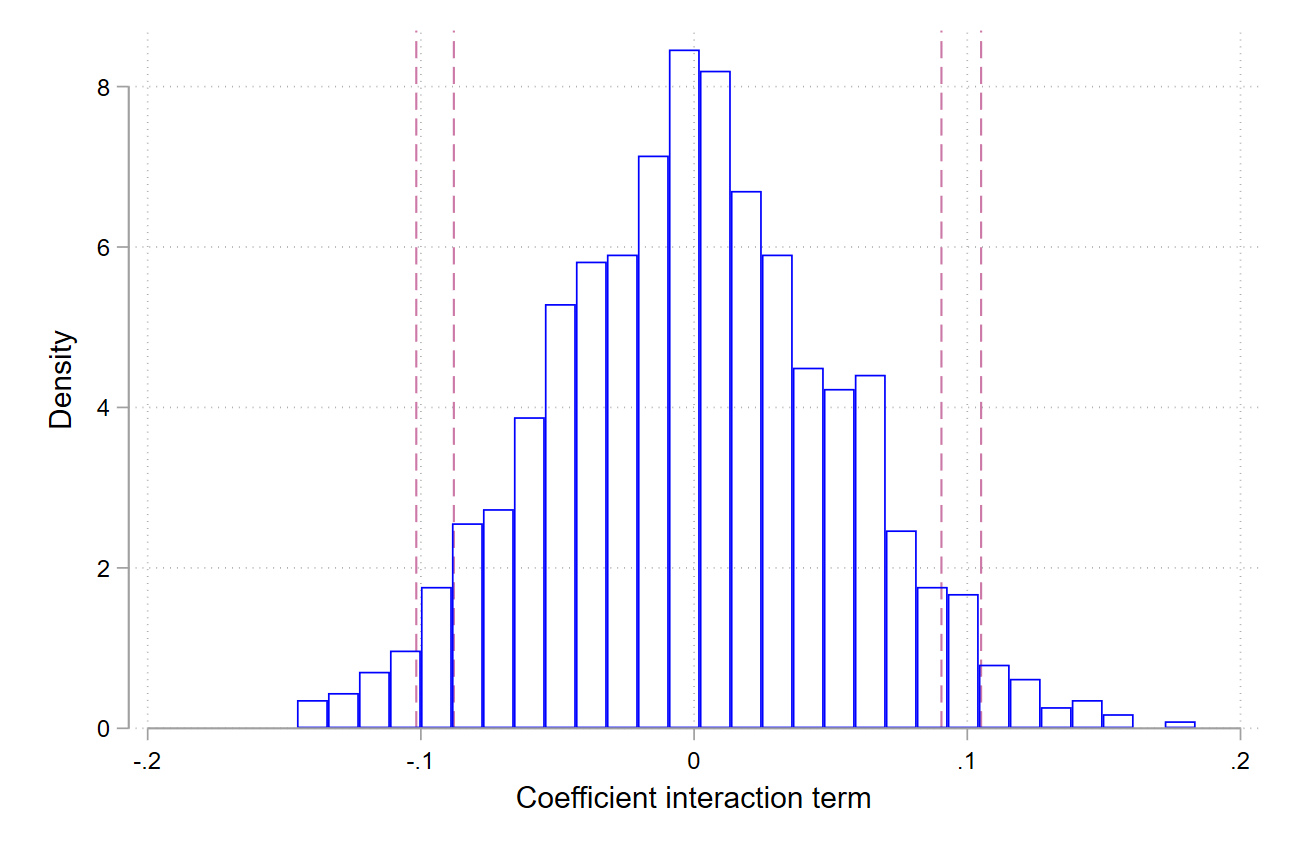
\includegraphics[width=0.9\linewidth]{../figures/permutation_coef_plink.png}
\caption{Permutation with Plink-based PGS (coef).}
\end{figure}

\begin{figure}[H]
\centering 
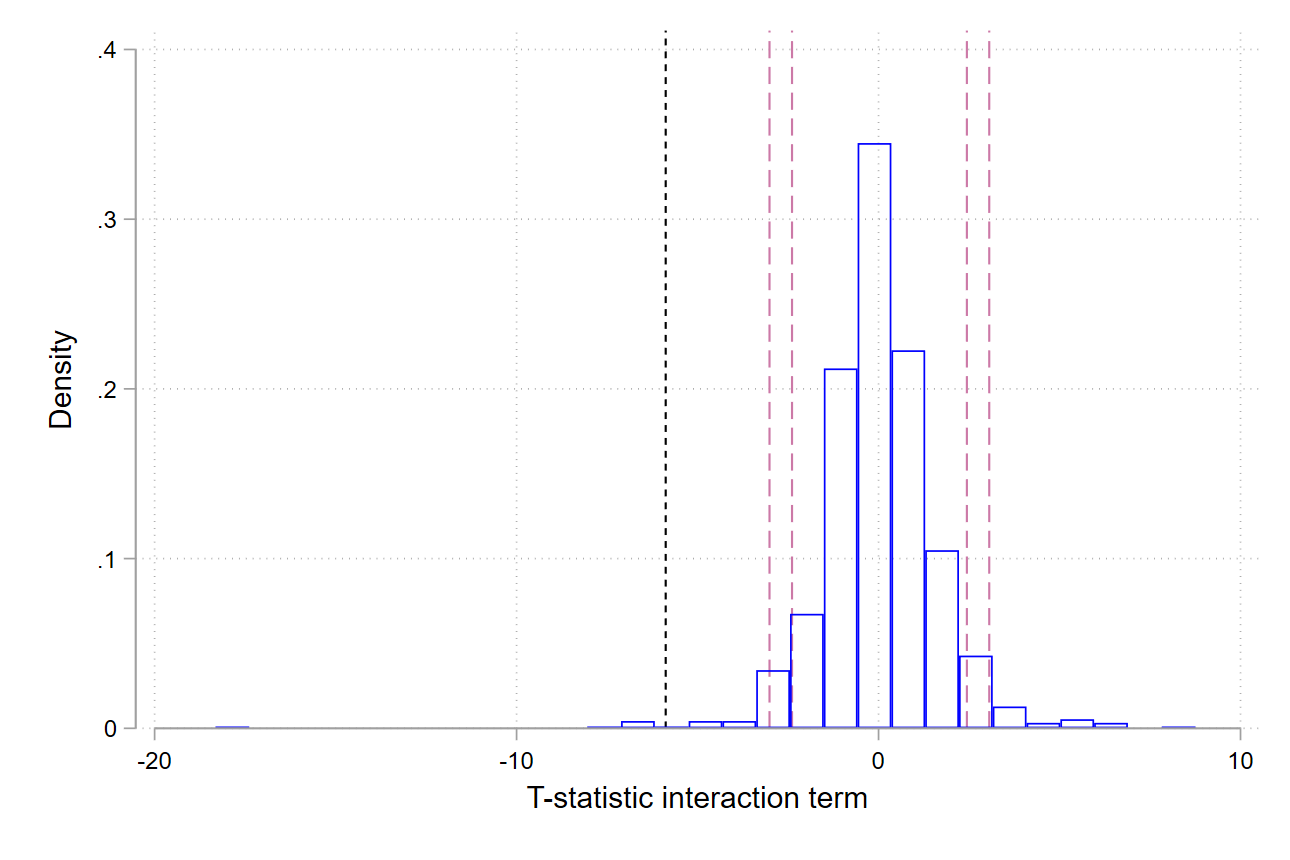
\includegraphics[width=0.9\linewidth]{../figures/permutation_tstat_plink.png}
\caption{Permutation with Plink-based PGS (t-stat).}
\end{figure}

%UKB
\begin{figure}[H]
\centering 
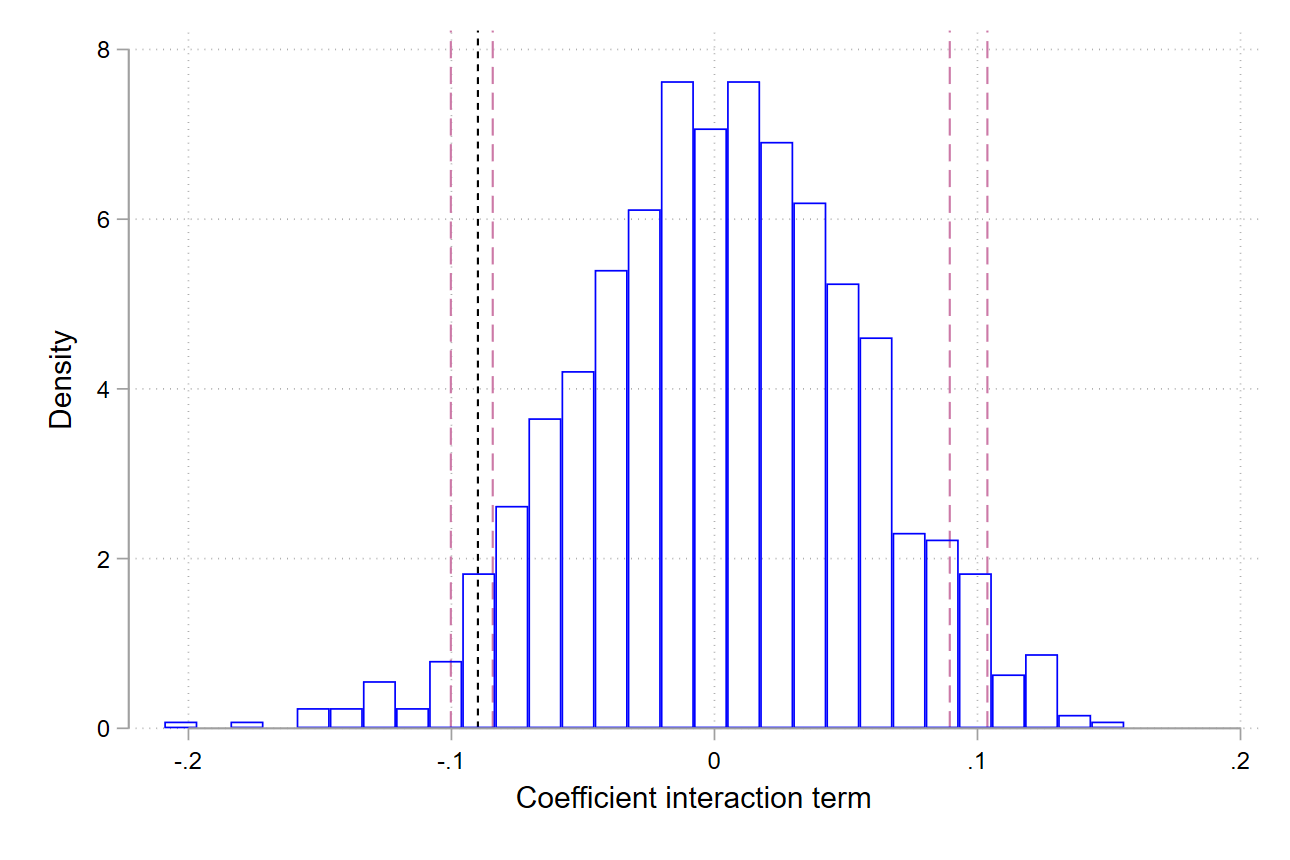
\includegraphics[width=1\linewidth]{../figures/permutation_coef_ukb.png}
\caption{Permutation with LDpred-based PGS - UKB (coef).}
\end{figure}

\begin{figure}[H]
\centering 
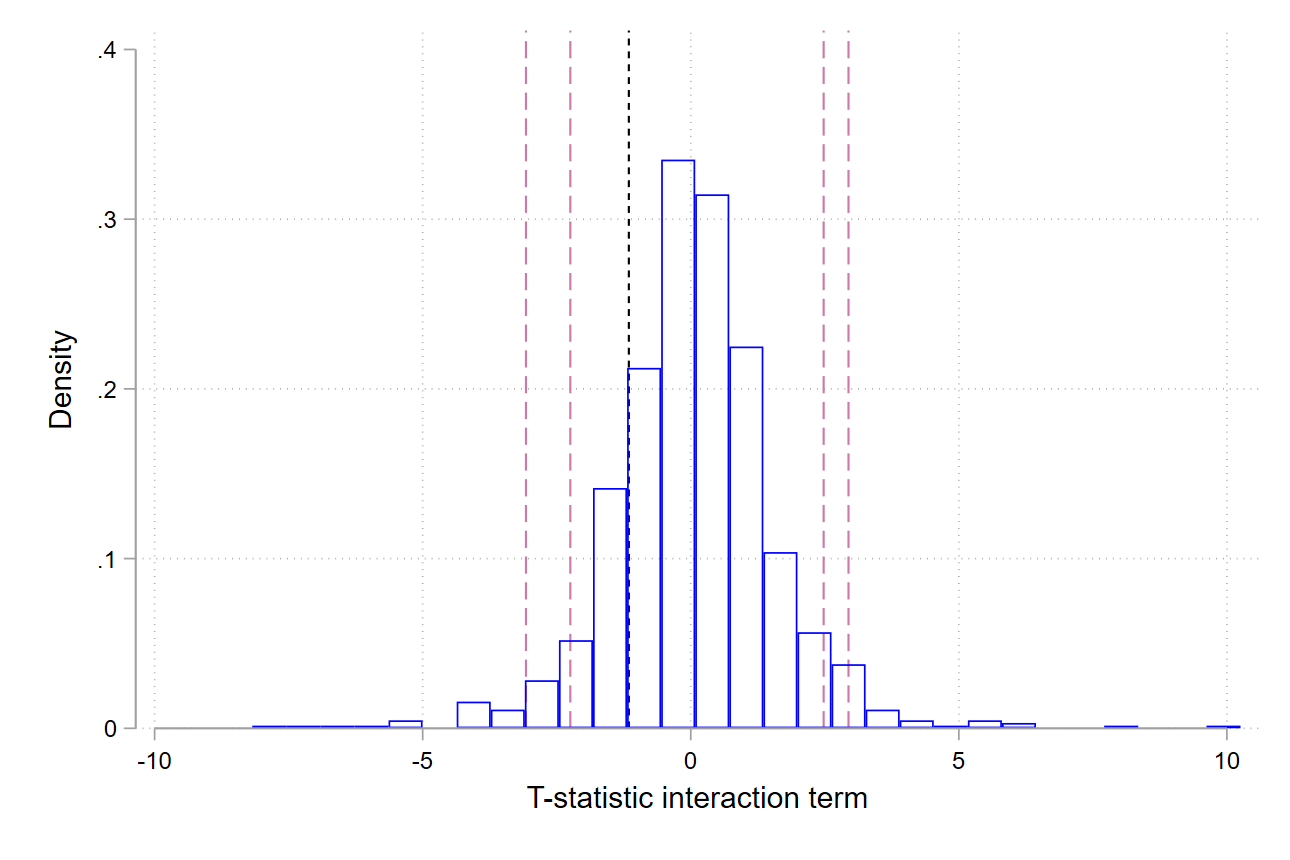
\includegraphics[width=1\linewidth]{../figures/permutation_tstat_ukb.png}
\caption{Permutation with LDpred-based PGS - UKB(t-stat).}
\end{figure}

%23me
\begin{figure}[H]
\centering 
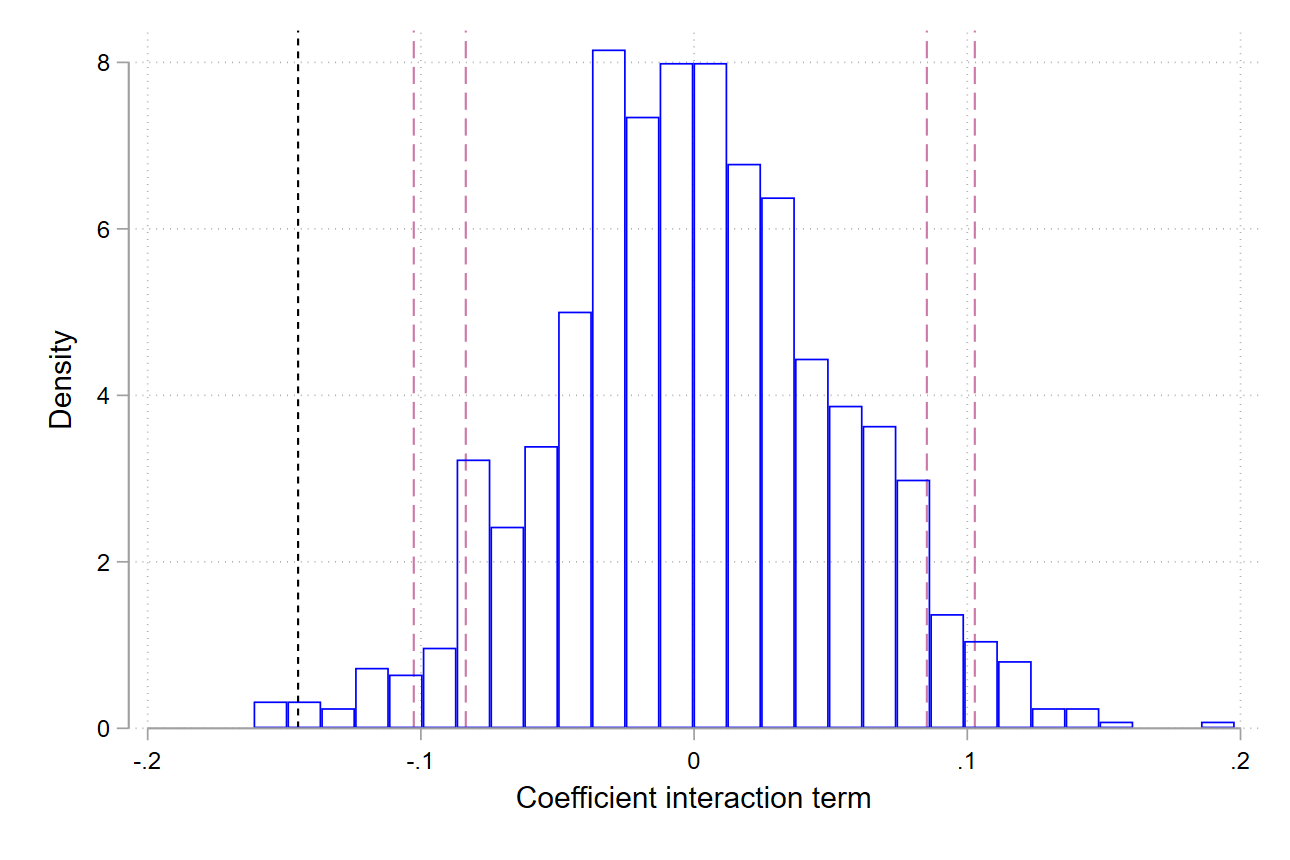
\includegraphics[width=1\linewidth]{../figures/permutation_coef_23me.png}
\caption{Permutation with LDpred-based PGS - 23me (coef).}
\end{figure}

\begin{figure}[H]
\centering 
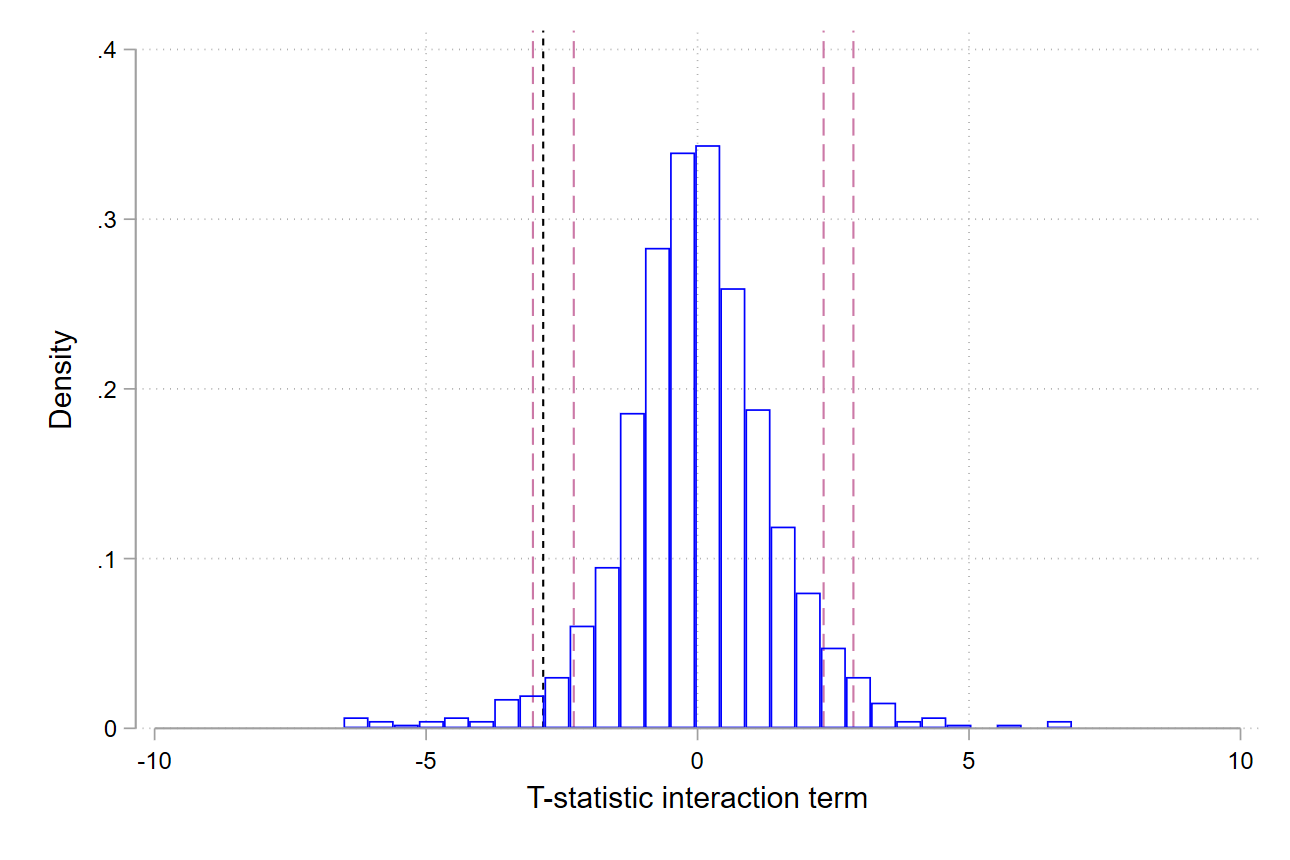
\includegraphics[width=1\linewidth]{../figures/permutation_tstat_23me.png}
\caption{Permutation with LDpred-based PGS - 23me (t-stat).}
\end{figure}


\end{document}

